\bibliographystyle{unsrt}
\nocite{*} %wszystkie wpisy trafią do bibliografii
\lstset{language=Java, tabsize=2,  basicstyle=\footnotesize\ttfamily, keywordstyle=\underbar}
\newgeometry{tmargin=3cm, bmargin=3cm, lmargin=2cm, rmargin=2cm}

\thispagestyle {empty}

\begin{center}
	%logo uczelni
	
\includegraphics[scale=0.4]{img/pw}
	
	\vspace{0.5cm}
	
	{\fontsize{20}{20}\selectfont POLITECHNIKA WARSZAWSKA}
	
	\vspace{1.0cm}
	
	\textbf{{\fontsize{14}{14}\selectfont Wydział Mechatroniki}}
	
	\vspace{1.5cm}
	
	\textbf{{\fontsize{14}{14}\selectfont Praca magisterska}}

	\vspace{2.0cm}
	
	{\fontsize{14}{14}\selectfont Konrad Traczyk}
	
	\vspace{1cm}
	
	{\fontsize{28}{28}\selectfont Projekt urządzenia do lokalizacji pojazdów w trybie on i off-line}
	
	\vspace{1cm}
	\begin{flushright}
		{\fontsize{14}{14}\selectfont Opiekun pracy: \\ 
		prof. dr hab. Michał Bartyś}
	
		\vspace{1cm}
		

		
	\end{flushright}
	
	\vspace{1cm}
	
	{\fontsize{12}{12}\selectfont Warszawa, 2017}
	
	%\cleardoublepage %nie działa
	
	%\clearpage\mbox{}\clearpage
\end{center}
\clearpage{\pagestyle{empty}\cleardoublepage}
\clearpage
\phantomsection
\addcontentsline{toc}{chapter}{Spis treści}
\tableofcontents
\clearpage
\phantomsection
\addcontentsline{toc}{chapter}{Spis rysunków}
\listoffigures
\clearpage
\chapter{Wstęp}
\label{ch:wstep}

\section{Zakres pracy}
\label{project_sketch}
Celem pracy był projekt, wykonanie i oprogramowanie urządzenia stanowiącego dodatkowe zabezpieczenie pojazdu na wypadek kradzieży, w postaci lokalizatora wykorzystującego system GNSS (\textit{ang. \textbf{G}lobal \textbf{N}avigation \textbf{S}atellite \textbf{S}ystem}) oraz GSM (\textit{ang. \textbf{G}lobal \textbf{S}ystem for \textbf{M}obile Communications}), zdolnego do analizy stylu jazdy kierowcy, a także systemu informatycznego, który pozwoliłby na przetworzenie pozyskanych danych. Poza nim, w skład systemu informatycznego wchodzą:

\begin{itemize}
\item Strona WWW, umożliwiająca zdalny podgląd danych pochodzących z przypisanych do użytkownika urządzeń.
\item Aplikacja serwerowa, która obsługuje zapytania użytkownika oraz zapisuje napływające dane do bazy danych SQLite.
\end{itemize}

Do dodatkowych wymagań stawianych urządzeniu należą:

\begin{itemize}
\item Zapewnienie bezpiecznego szyfrowanego kanału komunikacji deaktywującej tryb alarmu.
\item Zaoewnienie zastępczego źródła zasilania, umożliwiającego pracę przy wyłączonym silniku pojazdu, bądź w razie odłączenia akumulatora.
\item Konstrukcja urządzenia o niewielkich wymiarach w celu umożliwienia łatwego ukrycia w pojeździe. 
\end{itemize}

Moduł umożliwia działanie w dwóch trybach. Pierwszy z nich polega na cyklicznym wysyłaniu na serwer pozycji i parametrów trakcyjnych samochodu w trakcie jego ruchu. Dzięki temu, możliwa jest między innymi zdalna ocena stylu jazdy kierowcy.

Drugi tryb jest aktywny w trakcie postoju i stanowi system alarmowego powiadamiania właściciela pojazdu o jego przemieszczeniu na przykład w przypadku kradzieży.

W celu zapewnienia bezpieczeństwa, postanowiono zrealizować projekt w postaci dwóch urządzeń. Jedno z nich – płytka lokalizatora, umożliwiająca lokalizację pojazdu oraz wysyłanie danych na serwer. Drugi moduł stanowi układ deaktywujący, którego zadaniem jest wyłączenie trybu alarmu po uruchomieniu samochodu przez upoważnioną do tego osobę. Obie płytki komunikują się ze sobą poprzez protokół Bluetooh Low Energy, zapewniający energooszczędną wymianę danych. Pozwala to na zasilenie układu deaktywującego z niewielkiej baterii i jego nieprzerwaną pracę nawet przez kilka lat bez konieczności wymiany źródła zasilania. 
Ponadto, aby umożliwić  bezpieczną transmisję danych, niezbędne jest zastosowanie mechanizmu szyfrowania. W celu eliminacji ryzyka podsłuchania procesu wymiany klucza szyfrującego, oba urządzenia zostały wyposażone w moduł NFC (\textit{ang. \textbf{N}ear \textbf{F}ield \textbf{C}ommunication}), zapewniającego bezkontaktową komunikację na odległość do 10 cm.
\clearpage
\section{Schemat blokowy}
\label{Schemat_blokowy_urządzen}
Na przedstawionym rysunku \ref{fig:image_device_block_diagram} zaprezentowano blokowy schemat funkcjonalny urządzeń, które stanowią główną część sprzętową projektu - moduł płyty głównej oraz moduł dezaktywatora. 

\begin{figure}[h]
	\centering
	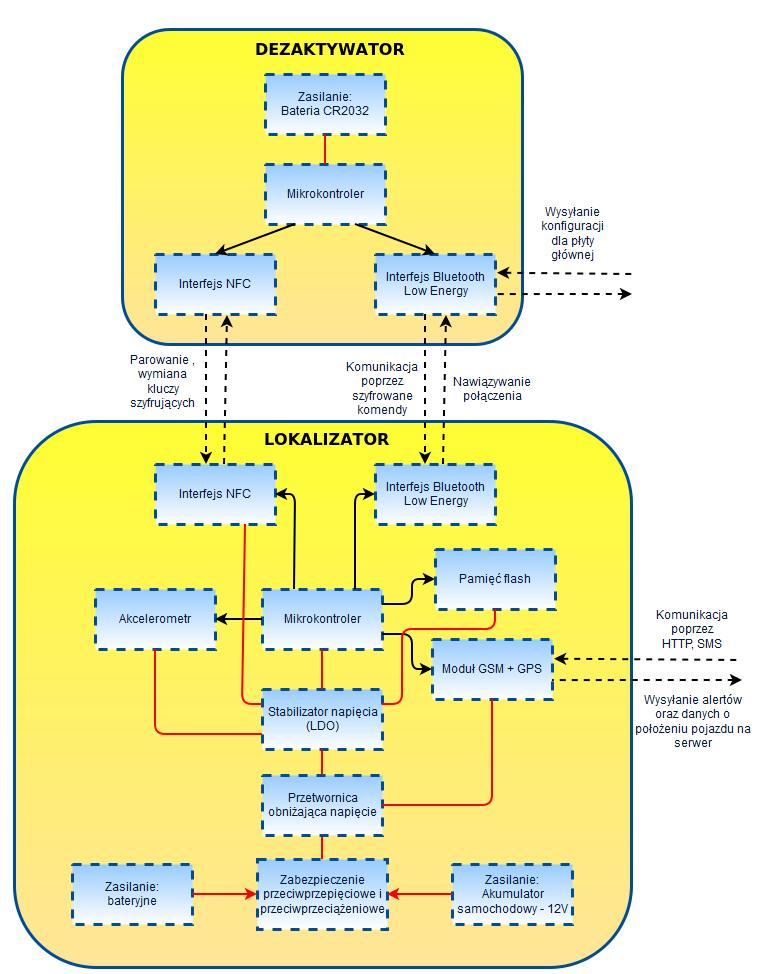
\includegraphics[width=13cm]{img/introduction/device_block_diagram.jpg}
	\caption{Schemat blokowy urządzeń wchodzących w skład systemu. \\ Źródło: Opracowanie własne.}
	\label{fig:image_device_block_diagram}
\end{figure}
	
	

\clearpage
\section{Istniejące rozwiązania}

W ramach pracy przeprowadzono analizę rynkową pod kątem istniejących, ciekawych rozwiązań. Poniżej zaprezentowano trzy najbardziej charakterystyczne z nich.

\begin{itemize}
\item Spark Nano 5.0 GPS Tracker

To przenośne urządzenie, posiadające zasilanie bateryjne i służące do śledzenia pozycji geograficznej przy pomocy systemu GPS. Zapewnia zdalne powiadamianie użytkownika o lokalizacji urządzenia poprzez sieć CDMA z dokładnością do 2m. Wymiary urządzenia: 64,5 x 40 x 20,5 mm. Urządzenie pozwala na działanie przez ok. 2 tygodnie, przy założeniu pracy przez 1 godzinę dziennie. Producent udostępnia platformę online oraz aplikacje na smartphony z systemem Android oraz IOS, do przedstawiania danych użytkownikowi. Urządzenie domyślnie raportuje położenie co minutę, lecz producent umożliwia zdalne zwiększenie częstotliwości w razie chęci użytkownika. Cena urządzenia: 129,99\$. Wizualizację urządzenia przedstawiono na rysunku \ref{fig:image_spark_nano_tracker}.
\begin{figure}[h]
	\centering
	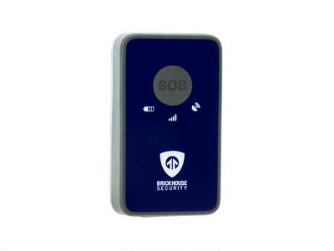
\includegraphics[width=7cm]{img/introduction/spark_nano.jpg}
	\caption{Spark Nano 5.0 GPS Tracker. Źródło: \cite{spark_nano}.}
	\label{fig:image_spark_nano_tracker}
\end{figure}

\item MyCarTracks - aplikacja mobilna

Jest to aplikacja na smartphona, która dodaje do niego funkcjonalność trackera GPS. Stanowi rozwiązanie typowo programowe, które wykorzystuje zasoby zawarte w telefonie – moduł GPS, GSM oraz internet. Jest ono proste i tanie, lecz nie pozbawione wad. Ponieważ to aplikacja na telefon, a nie osobne urządzenie, konieczne jest umieszczenie smartphone’a w pojeździe na stałe, jeśli użytkownik chciałby użytkować ją jako zabezpieczenie antykradzieżowe. Ponadto, telefony pobierają stosunkowo dużo energii co wymusza częste ich ładowanie. W rezultacie efektywne ukrycie urządzenia jest utrudnione. 
Do kosztów rozwiązania należy wliczyć cenę telefonu (używane urządzenie kosztuje ok. 200-300zł) oraz 7\$ za każdy pojazd miesięcznie. Aplikację przedstawiono na rysunku \ref{fig:image_my_car_tracks}.
\begin{figure}[h]
	\centering
	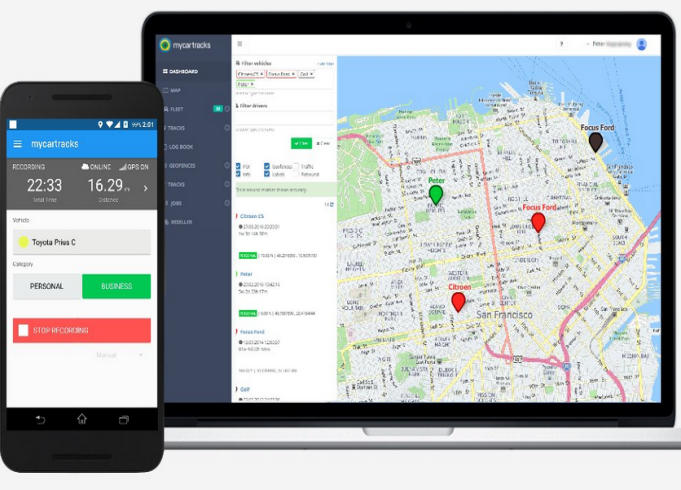
\includegraphics[width=7cm]{img/introduction/mycartracks.jpg}
	\caption{Aplikacja MyCarTracks. Źródło: \cite{my_car_tracks}.}
	\label{fig:image_my_car_tracks}
\end{figure}

\item STI GL300

Jest to kolejne niewielkie, przenośne urządzenie wykorzystujące moduł GPS do lokalizacji. Przekazuje ono informacje o położeniu w czasie rzeczywistym (co 60, 10 lub 5 sekund w zależności od wykupionej taryfy). Producent nie przedstawił informacji o sposobie komunikacji z serwerem, lecz najprawdopodobniej również wykorzystuje sieć GSM. Urządzenie to posiada baterię pozwalającą na ciągłą pracę do 2 tygodni. Przy tym nie ogranicza się ono jedynie do lokalizacji pojazdów dzięki niewielkim wymiarom. Producent wprowadza ciekawe funkcjonalności: powiadamianie poprzez wiadomość sms o osiągnięciu przez pojazd danej pozycji geograficznej, wejście w zdefiniowany obszar czy osiągnięcie pewnej prędkości. Aktualne oraz historyczne dane są przedstawiane użytkownikowi poprzez stronę internetową na mapach od firmy Google. Wymiary urządzenia to zaledwie ok. 5 cm x 2,5 cm x 2 cm.  W opcji dodatkowej można dokupić wodoodporną obudowę, pozwalającą na zamontowanie urządzenia na zewnątrz pojazdu. Cena urządzenia to 70\$ oraz od 25\$ do 40\$ miesięcznej opłaty. Wygląd urządzenia pokazano na rysunku \ref{fig:image_sti_gl300}.
\begin{figure}[h]
	\centering
	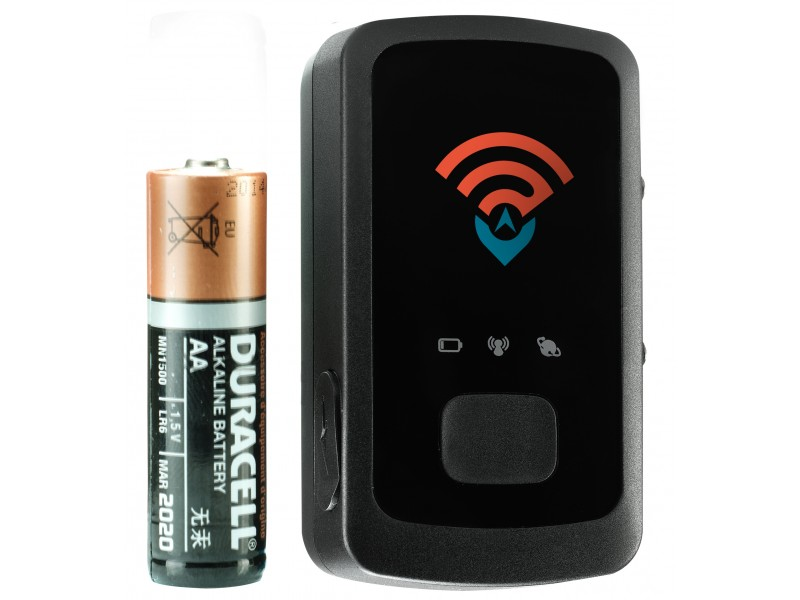
\includegraphics[width=7cm]{img/introduction/sti_gl300.jpg}
	\caption{Urządzenie STI GL300. Źródło: \cite{gl300}.}
	\label{fig:image_sti_gl300}
\end{figure}
\end{itemize}




\clearpage{\pagestyle{empty}\cleardoublepage}
\chapter{Propagacja sygnału radiowego w pomieszczeniu zamkniętym}
\label{ch:propagacja}
 

\clearpage{\pagestyle{empty}\cleardoublepage}
\chapter{Metody lokalizacji bezprzewodowej w pomieszczeniu}
\label{ch:metody-lokalizacji}

\section{Technologie radiowe}

\subsection{Wi-Fi}

\subsection{Bluetooth}
\subsubsection{Bluetooth Low Energy}

\section{Algorytmy}

\subsection{Trilateracja}

\subsection{Fingerprinting}



\clearpage{\pagestyle{empty}\cleardoublepage}
\chapter{Projekt algorytmu lokalizacji robota}
\label{ch:nrf}

\section{Gromadzenie danych ze znaczników}

\section{Filtracja i konwersja danych RSSI na odległość}

\section{Trilateracja}


 

\clearpage{\pagestyle{empty}\cleardoublepage}
\chapter{Projekt algorytmu fuzji sensorycznej}
\label{ch:fuzja}

\section{Fuzja sensoryczna}

\section{Filtr Kalmana}

\section{Filtr cząsteczkowy}

\section{Fuzja lokalizacji BLE z odometrią}

\section{Fuzja lokalizacji BLE z sensorem bezwładnościowym}

\section{Fuzja lokalizacji BLE z lokalizacją w oparciu o skaner laserowy}
 

\clearpage{\pagestyle{empty}\cleardoublepage}
\chapter{Platforma testowa}
\label{ch:platforma}

\section{System locationTAG}

\subsection{Znacznik locationTAG}

\subsection{System gromadzenia danych}


\section{Robot}

\clearpage{\pagestyle{empty}\cleardoublepage}
\chapter{Testy rozwiązania} 
\label{ch:testy}



\section{Narzędzia testowe}

\section{Porównanie metod filtracji siły sygnału RSSI}

\section{Porównanie metod fuzji sensorycznej}



\clearpage{\pagestyle{empty}\cleardoublepage}

\phantomsection
\addcontentsline{toc}{chapter}{Bibliografia}
\bibliographystyle{unsrt}	
\bibliography{bibliografia}
%\end{center}
\clearpage
\phantomsection
\addcontentsline{toc}{chapter}{Wykaz skrótów}
\chapter*{Wykaz skrótów}

\begin{tabular}{l l}
AES & Advanced Encryption Standard \\
API & Application Programming Interface \\
BLE & Bluetooth Low Energy \\
GATT & Generic Attibute \\
GCC & GNU Compiler Collection \\
GNSS & Global Navigation Satellite System \\
GPS & Global Positioning System \\
GSM & Global System for Mobile Communication \\
ISM & Industrial, Scientific, Medical (pasmo częstotliwości) \\
MAC & Media Access Control \\
RAM & Random Access Memory \\
RSSI & Radio Signal Strength Indicator \\
SDK & Software Development Kit \\
SMS & Short Message System \\
UHF & Ultra High Frequency \\




\end{tabular}

